%---------------------------------------------------------------------  
    \section{Resultados/Discusión}
    %------------------------------ SLIDE ---------------------------------------
    \begin{frame}{Resultados/Discusión} % cada entorno frame es una diapositiva
        \justifying % para justificar el texto, siempre al inicio de cada frame
        % Añade espacio para mover el bloque hacia arriba
        % Añade espacio para mover el bloque hacia arriba
        \vspace*{-0.3cm} % Ajusta este valor según sea necesario
        
        % Cuadro sin bordes redondeados, con colores personalizados
        \begin{tcolorbox}[colback=custombgcolor3, coltext=customfgcolor2,
                      colframe=custombgcolor3, % Color del borde
                      width=\textwidth,       % Ancho del cuadro
                      boxrule=1pt,            % Grosor del borde
                      top=1mm, bottom=1mm,     % Espacio superior e inferior
                      sharp corners=all,     % Bordes sin redondear
                      halign=center,         % Alineación horizontal
                      valign=center,         % Alineación vertical
                      ]
            % Texto dentro del cuadro
            %\textbf{Espectro \kern-0.5em de \kern-0.5em partículas \kern-0.5em a \kern-0.5em 7 m.s.n.m.}
            \textbf{Espectro de partículas a 7 m.s.n.m.}        
        \end{tcolorbox}
        
        \begin{figure}
            \centering
            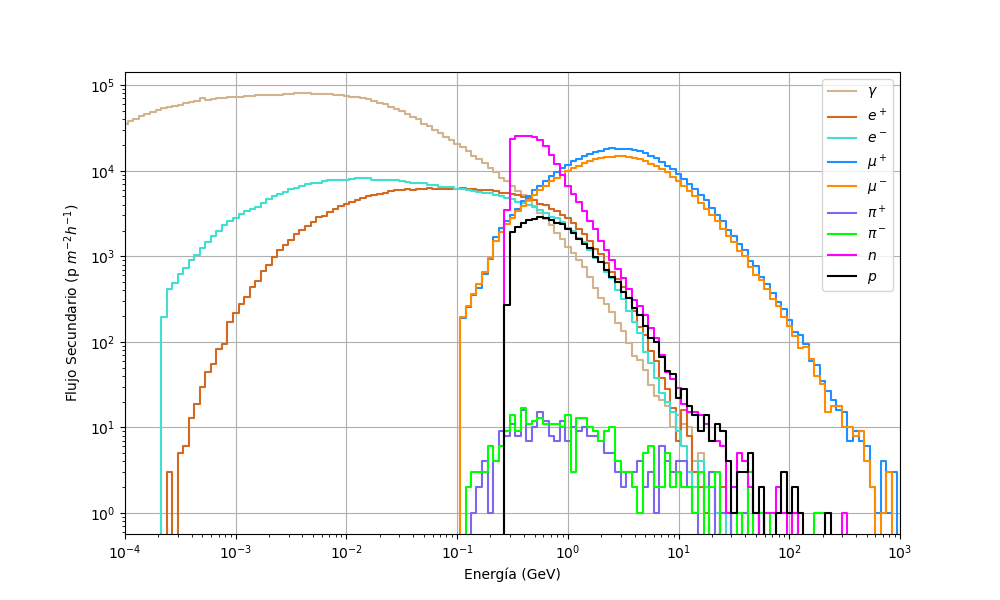
\includegraphics[width=0.6\textwidth]{Figures/Thesis_flux_new2_7msnm_without_title.png}
            \caption{\tiny Espectro de partículas secundarias obtenido a una altura de 7 m s.n.m.  Los colores corresponden a las diferentes partículas secundarias que lograron llegar al nivel de observación.}
        \end{figure}
    \end{frame}     
    
    %------------------------------ SLIDE ---------------------------------------
    \begin{frame}{} % cada entorno frame es una diapositiva
        \justifying % para justificar el texto, siempre al inicio de cada frame
        % Añade espacio para mover el bloque hacia arriba
        % Añade espacio para mover el bloque hacia arriba
        \vspace*{-0.2cm} % Ajusta este valor según sea necesario

        % Cuadro sin bordes redondeados, con colores personalizados
        \begin{tcolorbox}[colback=custombgcolor2, coltext=customfgcolor2,
                      colframe=custombgcolor2, % Color del borde
                      width=\textwidth,       % Ancho del cuadro
                      boxrule=1pt,            % Grosor del borde
                      top=1mm, bottom=1mm,     % Espacio superior e inferior
                      sharp corners=all,     % Bordes sin redondear
                      halign=center,         % Alineación horizontal
                      valign=center,         % Alineación vertical
                      ]
            % Texto dentro del cuadro
            %\textbf{Espectro \kern-0.5em de \kern-0.5em partículas \kern-0.5em a \kern-0.5em 7 m.s.n.m.}
            \textbf{Espectro de partículas a 4582.5 m.s.n.m.}        
        \end{tcolorbox}
        
        \begin{figure}
            \centering
            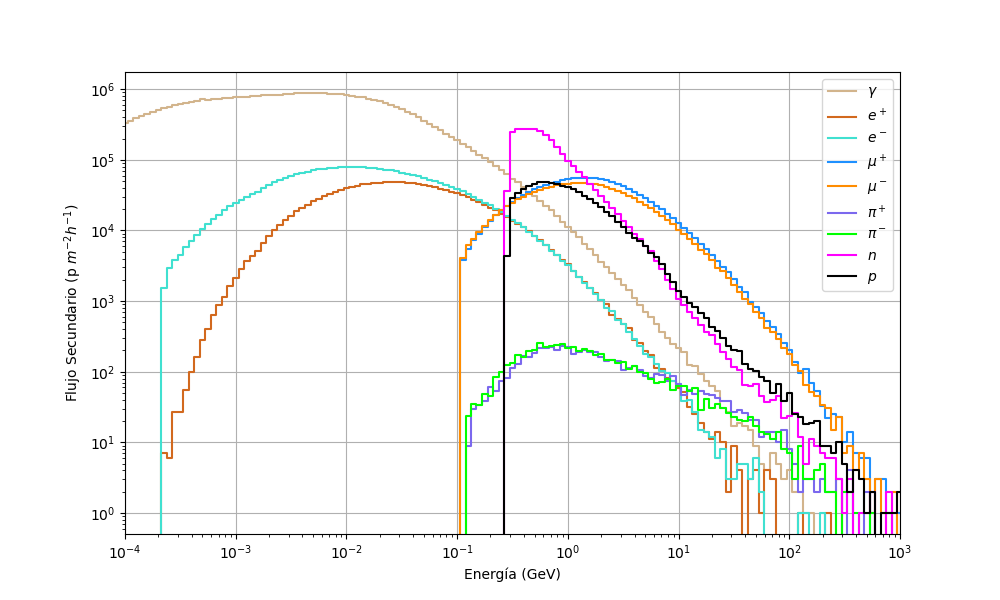
\includegraphics[width=0.6\textwidth]{Figures/Thesis_flux_new2_4600msnm_without_title.png}
            \caption{\tiny Espectro de partículas secundarias obtenido a una altura de 4582.5 m s.n.m. Los colores corresponden a las diferentes partículas secundarias que lograron llegar al nivel de observación.}
        \end{figure}
    \end{frame} 

    %------------------------------ SLIDE ---------------------------------------
    \begin{frame}{} % cada entorno frame es una diapositiva
        \justifying % para justificar el texto, siempre al inicio de cada frame
        % Añade espacio para mover el bloque hacia arriba
        % Añade espacio para mover el bloque hacia arriba
        \vspace*{-0.1cm} % Ajusta este valor según sea necesario

        % Cuadro sin bordes redondeados, con colores personalizados
        \begin{tcolorbox}[colback=custombgcolor4, coltext=customfgcolor2,
                      colframe=custombgcolor4, % Color del borde
                      width=\textwidth,       % Ancho del cuadro
                      boxrule=1pt,            % Grosor del borde
                      top=1mm, bottom=1mm,     % Espacio superior e inferior
                      sharp corners=all,     % Bordes sin redondear
                      halign=center,         % Alineación horizontal
                      valign=center,         % Alineación vertical
                      ]
            % Texto dentro del cuadro
            %\textbf{Espectro \kern-0.5em de \kern-0.5em partículas \kern-0.5em a \kern-0.5em 7 m.s.n.m.}
            \textbf{Flujo de neutrones con EXPACS}        
        \end{tcolorbox}
        
        \begin{figure}
            \centering
            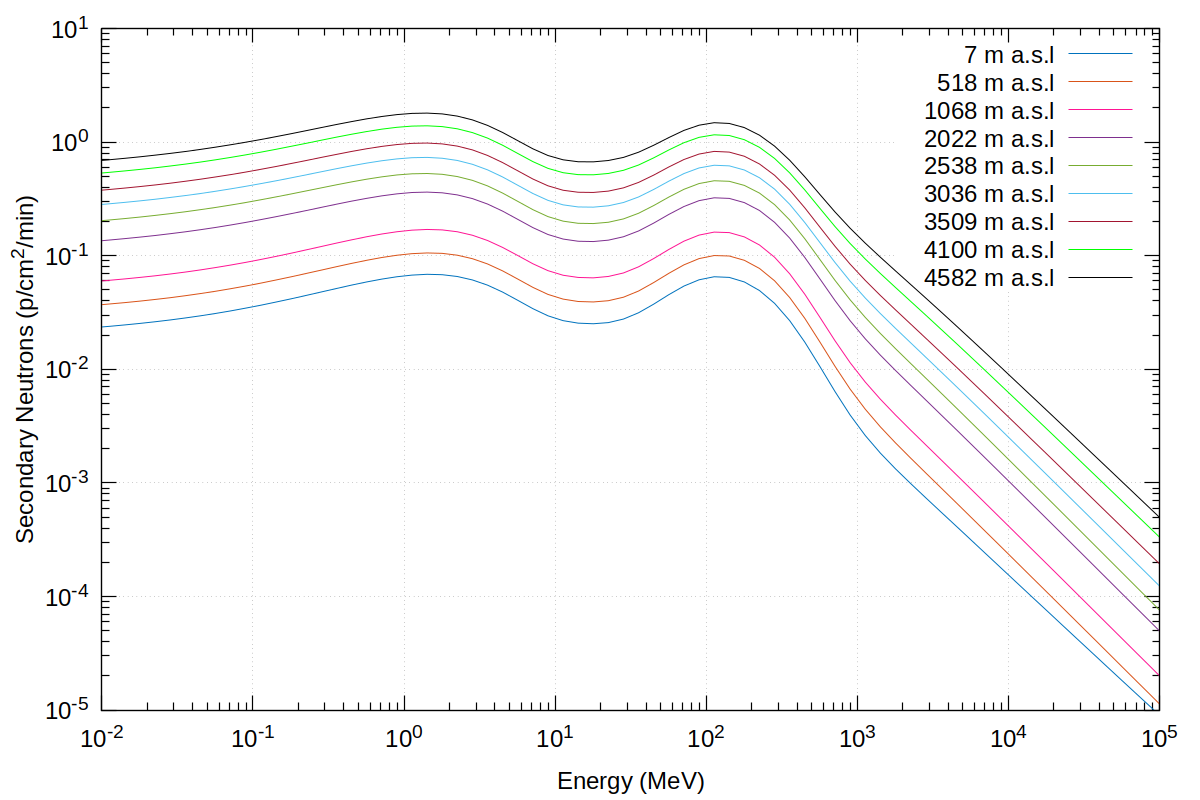
\includegraphics[width=0.55\textwidth]{Figures/Neutron_flux.png}
            \caption{\tiny Espectro de neutrones a diferentes alturas utilizando EXPACS [\cite{sedrati2022}].}
        \end{figure}
    \end{frame}

    %------------------------------ SLIDE ---------------------------------------
    \begin{frame}{} % cada entorno frame es una diapositiva
        \justifying % para justificar el texto, siempre al inicio de cada frame
        % Añade espacio para mover el bloque hacia arriba
        % Añade espacio para mover el bloque hacia arriba
        \vspace*{-0.2cm} % Ajusta este valor según sea necesario

        % Cuadro sin bordes redondeados, con colores personalizados
        \begin{tcolorbox}[colback=custombgcolor8, coltext=customfgcolor2,
                      colframe=custombgcolor8, % Color del borde
                      width=\textwidth,       % Ancho del cuadro
                      boxrule=1pt,            % Grosor del borde
                      top=1mm, bottom=1mm,     % Espacio superior e inferior
                      sharp corners=all,     % Bordes sin redondear
                      halign=center,         % Alineación horizontal
                      valign=center,         % Alineación vertical
                      ]
            % Texto dentro del cuadro
            %\textbf{Espectro \kern-0.5em de \kern-0.5em partículas \kern-0.5em a \kern-0.5em 7 m.s.n.m.}
            \textbf{Flujo de protones y neutrones vs altura}        
        \end{tcolorbox}
        
        \begin{figure}
            \centering
            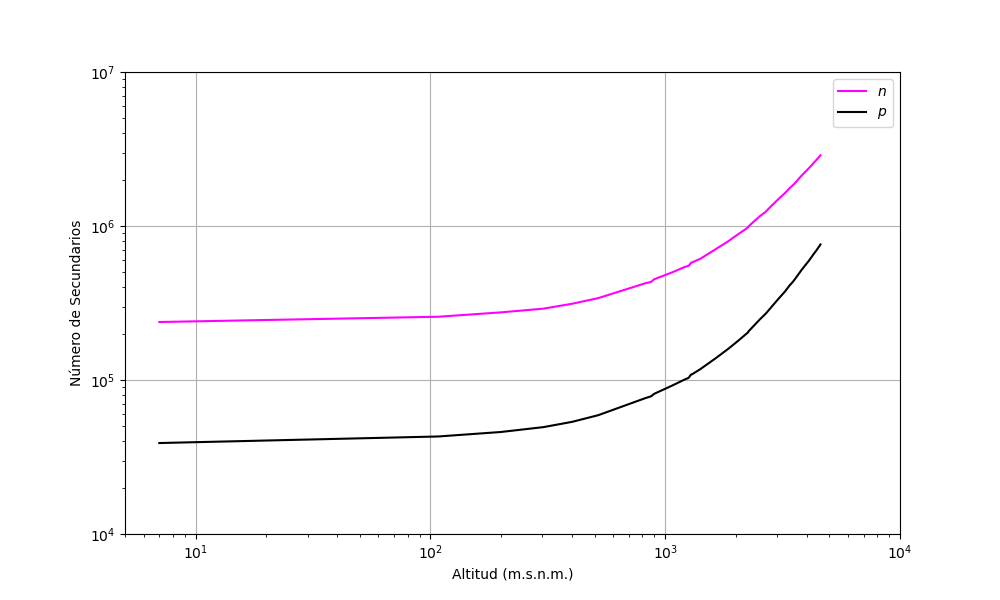
\includegraphics[width=0.6\textwidth]{Figures/Thesis_flux_protons_and_neutrons.png}
            \caption{\tiny Flujo total de protones (negro) y neutrones (rosa) desde nivel del mar hasta cima del volcán Sierra Negra ($4582$.5 m s.n.m.) obtenido a través de las simulaciones con CORSIKA.}
        \end{figure}
    \end{frame} 
    
    %------------------------------ SLIDE ---------------------------------------
    \begin{frame}{} % cada entorno frame es una diapositiva
        \justifying % para justificar el texto, siempre al inicio de cada frame
        % Añade espacio para mover el bloque hacia arriba
        % Añade espacio para mover el bloque hacia arriba
        \vspace*{-0.1cm} % Ajusta este valor según sea necesario

        % Cuadro sin bordes redondeados, con colores personalizados
        \begin{tcolorbox}[colback=custombgcolor9, coltext=customfgcolor2,
                      colframe=custombgcolor9, % Color del borde
                      width=\textwidth,       % Ancho del cuadro
                      boxrule=1pt,            % Grosor del borde
                      top=1mm, bottom=1mm,     % Espacio superior e inferior
                      sharp corners=all,     % Bordes sin redondear
                      halign=center,         % Alineación horizontal
                      valign=center,         % Alineación vertical
                      ]
            % Texto dentro del cuadro
            %\textbf{Espectro \kern-0.5em de \kern-0.5em partículas \kern-0.5em a \kern-0.5em 7 m.s.n.m.}
            \textbf{Número de cuentas registrado con el MMN}        
        \end{tcolorbox}
        
        \begin{figure}
            \centering
            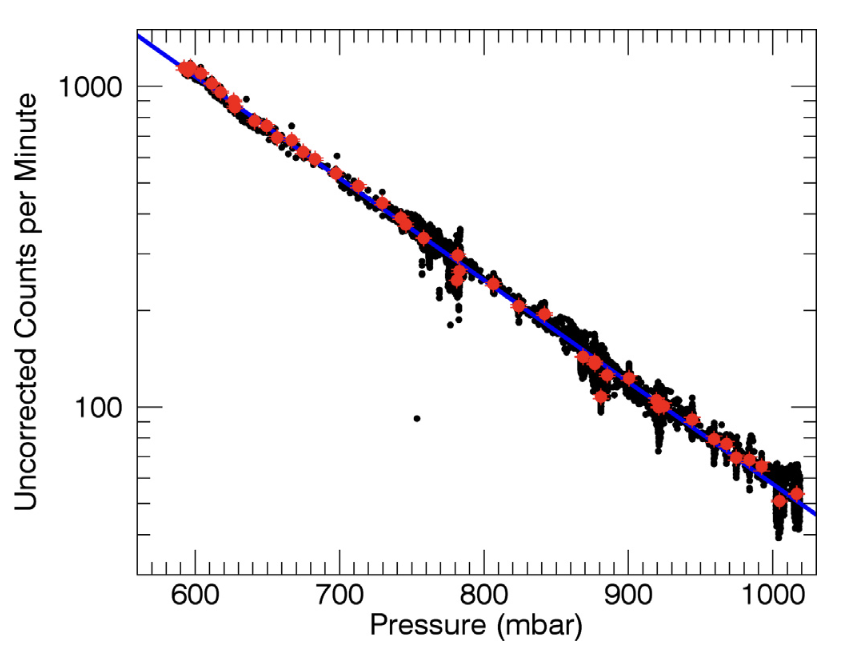
\includegraphics[width=0.45\textwidth]{Figures/rate-MMN.png}
            \caption{\tiny Número de cuentas por minuto en función de la presión observada registrada por el MMN. Estudio realizado por \cite{lara2016}.}
        \end{figure}
    \end{frame}    